\documentclass[journal, onecolumn, 12pt]{IEEEtran}

% Packages
\usepackage{cite}
\usepackage{amsmath,amssymb,amsfonts}
\usepackage{algorithmic}
\usepackage{graphicx}
\usepackage{textcomp}
\usepackage{xcolor}
\usepackage{booktabs} % For nicer tables
\usepackage{multirow} % For multi-row cells
\usepackage{listings} % For code inclusion
\usepackage{geometry}
\usepackage[table]{xcolor}
\usepackage{placeins}

% Custom pastel colors for readability
\definecolor{mygreen}{rgb}{0.7, 1, 0.7}   % Light Green
\definecolor{myyellow}{rgb}{1, 1, 0.7}    % Light Yellow
\definecolor{myred}{rgb}{1, 0.7, 0.7}     % Light Red

% Page margins adjustment for homework readability
\geometry{letterpaper, top=1in, bottom=1in, left=1in, right=1in}

% Code listing style
\definecolor{codegreen}{rgb}{0,0.6,0}
\definecolor{codegray}{rgb}{0.5,0.5,0.5}
\definecolor{codepurple}{rgb}{0.58,0,0.82}
\definecolor{backcolour}{rgb}{0.95,0.95,0.92}

\lstdefinestyle{mystyle}{
    backgroundcolor=\color{backcolour},   
    commentstyle=\color{codegreen},
    keywordstyle=\color{magenta},
    numberstyle=\tiny\color{codegray},
    stringstyle=\color{codepurple},
    basicstyle=\ttfamily\footnotesize,
    breakatwhitespace=false,         
    breaklines=true,                 
    captionpos=b,                    
    keepspaces=true,                 
    numbers=left,                    
    numbersep=5pt,                  
    showspaces=false,                
    showstringspaces=false,
    showtabs=false,                  
    tabsize=2
}

\lstset{style=mystyle}

% Title Information
\title{ECE275: Homework \#1}
\author{John R. Minnick\\
ECE 275: Electricity Market, Policy, and Modeling \\
Department of Electrical and Computer Engineering\\
February, 2026\\
\thanks{\textbf{Disclaimer:} Generative AI was used for the creation of the structure of this document as well as in some of the implementation of the underlying code used for modeling. However all written content and opinions on matters here within are solely those of the author.}
}

\begin{document}

\maketitle

\section{The Role of Modeling in Policy }

\subsection{Guideline Criteria for Quantification}

For the purposes of evaluating whether the following policy questions are suited for modeling based analysis, we shall utilize the guideline criteria provided in Table \ref{tab:pocket_guide} as shown below.
    
\begin{table}[h]
\caption{A Pocket Guide to Quantification (Adapted from Reading)}
\label{tab:pocket_guide}
\centering
\begin{tabular}{@{}p{2.5cm}p{2.5cm}p{2.5cm}p{2.5cm}p{2.5cm}p{2.5cm}@{}}
\toprule
\textbf{Criterion \textbackslash Suitability} & \textbf{High } & \textbf{Medium} & \textbf{Low} & \textbf{None} & \textbf{Negative} \\ \midrule
\textbf{Morality} & Amoral issues & Minor moral relevance & Moral issue to few & Moral issue to many & Clear moral issue \\ \addlinespace
\textbf{Political Principle} & Apolitical issue & Weak implications & Political overtones & Major political position & Prime political position \\ \addlinespace
\textbf{Emotional Level} & None & Special interest groups only & Headlines in tabloids & Headlines in established press & Catastrophic event \\ \addlinespace
\textbf{Statutory Constraint} & Clearly required & Clearly implied & Allowed & Not mentioned & Prohibited / No consensus \\ \addlinespace
\textbf{Level of Consensus} & High & Two positions & Three positions & Five positions & --- \\ \addlinespace
\textbf{Number of Actors} & One & Five & Ten & Twenty & Dozens \\ \addlinespace
\textbf{Decision Level} & Staff & Manager & Third-level executive & Second-level executive & Chief Executive \\ \addlinespace
\textbf{Complexity \& Knowledge} & Few relevant factors; Traditional physical systems & Many factors, most understood; New physical systems & Many factors, few understood; Research completed & Several years of research underway; Anecdotes only & No understanding; Strictly legal issues \\ \addlinespace
\textbf{Available Data} & Current, long-term, continuous & Long-term, intermittent & Recent data only & Anecdotal data only & None \\ \bottomrule
\end{tabular}
\end{table}


\newpage

\subsection{Part A: Mountain-top Removal}
\textit{Prompt: Should mountain-top removal for coal mining be prohibited?}\\

The question of whether mountain-top removal for coal mining should be prohibited  \textbf{is not suitable for modeling-based analysis.} By evaluating this policy question  using the guideline criteria in Table \ref{tab:pocket_guide}, we find the following:

% --- PASTE THIS IN YOUR DOCUMENT BODY ---

% TABLE 1A: MOUNTAIN-TOP REMOVAL
% Analysis: High moral/emotional content, low consensus, highly political.
% Result: Mostly RED.
\begin{table}[h]
    \caption{Quantification Guide: Part A (Mountain-top Removal)}
    \label{tab:guide_part_a}
    \centering
    \begin{tabular}{@{}p{2.5cm}p{2.5cm}p{2.5cm}p{2.5cm}p{2.5cm}p{2.5cm}@{}}
    \toprule
    \textbf{Criterion \textbackslash Suitability} & \textbf{High } & \textbf{Medium} & \textbf{Low} & \textbf{None} & \textbf{Negative} \\ \midrule
    
    \textbf{Morality} & Amoral issues & Minor moral relevance & Moral issue to few & \cellcolor{myred} Moral issue to many &  Clear moral issue \\ \addlinespace
    
    \textbf{Political Principle} & Apolitical issue & Weak implications & Political overtones & Major political position & \cellcolor{myred} Prime political position \\ \addlinespace
    
    \textbf{Emotional Level} & None & Special interest groups only & Headlines in tabloids & \cellcolor{myred} Headlines in established press &  Catastrophic event \\ \addlinespace
    
    \textbf{Statutory Constraint} & \cellcolor{mygreen} Clearly required & Clearly implied & Allowed & Not mentioned &  Prohibited / No consensus \\ \addlinespace
    
    \textbf{Level of Consensus} & High & \cellcolor{mygreen} Two positions & Three positions & Five positions & --- \\ \addlinespace
    
    \textbf{Number of Actors} & One & Five & Ten & Twenty & \cellcolor{myred} Dozens \\ \addlinespace
    
    \textbf{Decision Level} & Staff & Manager & Third-level executive & Second-level executive & \cellcolor{myred} Chief Executive \\ \addlinespace
    
    \textbf{Complexity \& Knowledge} & Few relevant factors & Many factors, most understood & \cellcolor{myyellow} Many factors, few understood & Research underway & No understanding \\ \addlinespace
    
    \textbf{Available Data} & Current, long-term & Long-term, intermittent & \cellcolor{myyellow} Recent data only & Anecdotal data only & None \\ \bottomrule
    \end{tabular}
\end{table}

There is a moral issue for many: most believe that prohibition of the removal of mountains tops is important, but not a moral right. This type of prohibition is rife with political tension, and thus sets itself as a prime political position. If such a policy were to be instated, it would most definitely dominate the news cycle in the established press. It also very clearly establishes the necessity of a statutory constraint via its seeking of a prohibitory measure. The level of consensus is medium, as some people want to preserve the environment while others rely on mining and coal industry for their livelihood. The numbers of actors is dozens for this policy, ranging from numerous environmentalist groups, the coal mining industry, the energy sector, the railroad and transportation sector, as well as several governmental agencies who would have input on its impact. The decision level for such a policy could only be determined at the highest levels of the government, most likely falling to a decision made in the congressional branch and upheld by the executive branch or vice-versa. For the complexity and knowledge, the impact of such a policy can be theorized but only the test of time would truly provide meaningful insight into the effects of mountain-top removal prohibition. Finally, data for such a policy is sparse. No policy has ever been passed that prohibits mountain-top removal. Some countries have restricted it while others have been able to phase it out via energy alternatives; but the impact of a prohibitive policy is speculative at best. \par
Thus, the question of whether mountain-top removal for coal mining should be prohibited \textbf{is not suitable for modeling-based analysis.} \\

However, if this policy where to be modeled the inputs and outputs could look something like the following: \\

\textbf{Inputs:}
\begin{itemize}
    \item Current coal production from mountain-top removal mining. 
    \item Cost of alternative energy sources.
    \item Cost of environmental restoration. 
    \item Alternative economic viability of local mining communities. \\
    
\end{itemize}


\textbf{Outputs:}
\begin{itemize}
  \item Impact on coal mining industry and adjacent businesses (Freight \& Refining).
  \item Impact on coal mining communities (Jobs, Infrastructure, \& Local Tax Revenue).
  \item Impact on electricity and heating prices.
  \item Impact on environmental conditions.\\
\end{itemize}

Modeling with these specific outputs in mind would allow us to make an informed and optimal policy decision. 

% YOUR ANSWER HERE
% Discuss applying the Table 5-1 framework. 
% Is it moral/political? 
% Define Inputs (data needed) and Outputs (results provided).
\newpage
\subsection{Part B: CO$_2$ Reduction Allocation}
\textit{Prompt: How should 40\% CO$_2$ reductions be allocated between mobile and stationary sources?}\\

The question of how \%40 CO$_2$ reductions should be allocated between mobile and stationary sources \textbf{is suitable for modeling-based analysis.} By evaluating this policy question  using the guideline criteria in Table \ref{tab:pocket_guide}, we find the following:

% TABLE 1B: CO2 REDUCTION ALLOCATION
% Analysis: Statutory requirement exists, technical "optimization" problem.
% Result: Mostly GREEN/YELLOW.
\begin{table}[h]
    \caption{Quantification Guide: Part B (CO$_2$ Allocation)}
    \label{tab:guide_part_b}
    \centering
    \begin{tabular}{@{}p{2.5cm}p{2.5cm}p{2.5cm}p{2.5cm}p{2.5cm}p{2.5cm}@{}}
    \toprule
    \textbf{Criterion \textbackslash Suitability} & \textbf{High} & \textbf{Medium} & \textbf{Low} & \textbf{None} & \textbf{Negative} \\ \midrule
    
    \textbf{Morality} & Amoral issues & \cellcolor{mygreen} Minor moral relevance & Moral issue to few & Moral issue to many & Clear moral issue \\ \addlinespace
    
    \textbf{Political Principle} & Apolitical issue & Weak implications & \cellcolor{myyellow} Political overtones & Major political position & Prime political position \\ \addlinespace
    
    \textbf{Emotional Level} & None & \cellcolor{mygreen} Special interest groups only & Headlines in tabloids & Headlines in established press & Catastrophic event \\ \addlinespace
    
    \textbf{Statutory Constraint} & \cellcolor{mygreen} Clearly required & Clearly implied & Allowed & Not mentioned & Prohibited / No consensus \\ \addlinespace
    
    \textbf{Level of Consensus} & High & Two positions & \cellcolor{myyellow} Three positions & Five positions & --- \\ \addlinespace
    
    \textbf{Number of Actors} & One & Five & \cellcolor{myyellow} Ten & Twenty & Dozens \\ \addlinespace
    
    \textbf{Decision Level} & Staff & Manager & \cellcolor{myyellow} Third-level executive & Second-level executive & Chief Executive \\ \addlinespace
    
    \textbf{Complexity \& Knowledge} & \cellcolor{mygreen} Traditional physical systems & Many factors, most understood & Many factors, few understood & Research underway & No understanding \\ \addlinespace
    
    \textbf{Available Data} & \cellcolor{mygreen} Current, long-term & Long-term, intermittent & Recent data only & Anecdotal data only & None \\ \bottomrule
    \end{tabular}
\end{table}
\FloatBarrier
Due to the question being \textit{how} CO$_2$ reductions should be allocated and not \textit{if} CO$_2$ should be allocated, the question holds little moral weight. Additionally, due to the hyper-specific nature of the policy, it cares slight political overtones but nothing that would dominate a news cycle. Only special interest groups would concern themselves with specific allocations, as this is typically not the concern of the common person. A statutory constraint is required as this policy would set restrictions in place as to where and how much CO$_2$ emissions can be generated. The level of consensus is quite low as people may have differing opinions about allocations, but the overall options are mobile-heavy, stationary-heavy, or roughly equal; thus three positions. Again, due to the hyper specific nature of this policy deal with allocation, it would most likely happen at the mid-range executive level. The complexity and knowledge of this topic is quite well known as CO$_2$ emissions and reductions are well tracked and the dynamics of the system are quite well know. Addtionally, there is a wealth of both current and long-term data available to model such a policy, thus further lending itself towards numerical analysis.\par
Thus, the question of how \%40 CO$_2$ reductions should be allocated between mobile and stationary sources \textbf{is suitable for modeling-based analysis.} \\

If this policy where to be modeled the inputs and outputs could look something like the following: \\
 
\textbf{Inputs:}
\begin{itemize}
    \item Current emission levels in both sectors.
    \item Total reduction target.
    \item Marginal cost curves for reducing CO$_2$ in stationary vs. mobile sources.
    \item Future extrapolation of CO$_2$ emission trajectory based on previous production trends.\\
\end{itemize}

\textbf{Outputs:}
\begin{itemize}
    \item The marginal cost of carbon abatement. 
    \item The optimal and semi-optimal splits which minimize economic cost.
    \item Adjusts to the splits to maintain optimization in future markets. \\ 
\end{itemize}

Modeling with these specific outputs in mind would allow us to make an informed and optimal policy decision. 

\newpage
\section{Linear Programming Practice}

\subsection{Problem Formulation}
The objective is to minimize the annual cost of operation for three power plants (Oil, Diesel, Hydro) across two demand periods.

\subsection{Part A: Unconstrained Dispatch}
\textbf{Primal Solution:}
\begin{itemize}
    \item Period 1 Generation: Oil: 400 MW, Diesel: 190 MW, Hydro: 100 MW
    \item Period 2 Generation: Oil: 200 MW, Diesel: 0 MW, Hydro: 100 MW
\end{itemize}

\textbf{Dual Variables (Marginal Costs):}
\begin{itemize}
    \item Period 1 Marginal Cost: \$130.00 / MWh
    \item Period 2 Marginal Cost: \$90.00 / MWh
\end{itemize}

\subsection{Part B: Hydro Energy Constraint}
The model was re-solved with a constraint of 320,000 MWh/year for the hydro plant.

\textbf{Total Cost:}\$327,280,000.00

\textbf{Primal Solution:}
\begin{itemize}
    \item Period 1 Generation: Oil: 400 MW, Diesel: 190 MW, Hydro: 100 MW
    \item Period 2 Generation: Oil: 293 MW, Diesel: 0 MW, Hydro: 7 MW
\end{itemize}

\textbf{Dual Variables (Marginal Costs):}
\begin{itemize}
    \item Period 1 Marginal Cost: \$130.00 / MWh
    \item Period 2 Marginal Cost: \$90.00 / MWh\\
    \item Hydro Energy Shadow Price: \$ -90.00/MWh
\end{itemize}

The model chooses to prioritize Period 1 because the savings are higher: \$130 > \$90. Thus, we run Hydro at full capacity during peak hours. We then use the remaining Hydro not consumed by our peak hours up-time to displace Oil during Period 2. 


\FloatBarrier
\begin{figure}[h]
    \centering
    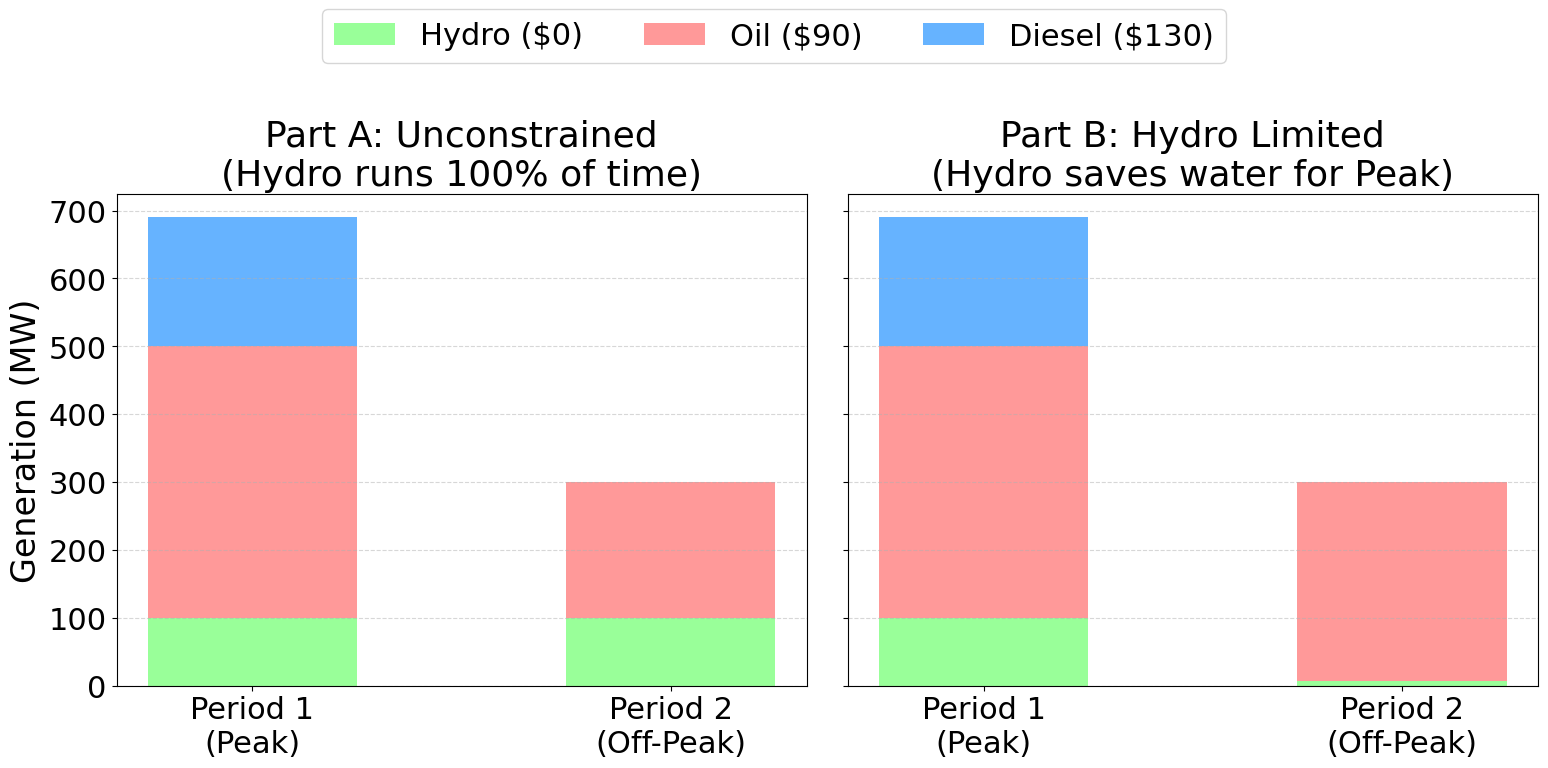
\includegraphics[width=0.6\textwidth]{ece275hw1p2.png}
    \caption{Optimal generation dispatch for Part A (Unconstrained) and Part B (Hydro Limited). In the unconstrained case (left), the zero-marginal-cost hydro plant (green) runs at full capacity in both periods. In the constrained case (right), the model conserves the limited hydro budget for Period 1 to displace the most expensive fuel (Diesel), reducing hydro output in Period 2 where it would only displace cheaper Oil.}
    \label{fig:dispatch_comparison}
\end{figure}
\FloatBarrier



\section{Appendix: Python Code}
\begin{lstlisting}[language=Python, caption=Power Plant Dispatch Optimization Code]
import numpy as np
from scipy.optimize import linprog
import matplotlib.pyplot as plt

def solve_and_analyze():
    """
    ECE275 Homework 1: Power Plant Dispatch Optimization
    
    This script solves two Linear Programming problems:
    1. Part A: Economic Dispatch with no energy constraints (Standard Merit Order).
    2. Part B: Economic Dispatch with a limited Hydro energy budget (Energy Limited).
    
    It outputs the Primal Solution (MW Generation) and Dual Variables (Marginal Costs)
    and generates a stacked bar chart comparison.
    """
    print("--- ECE275 Homework 1: Power Dispatch Optimization ---\n")

    # ==========================================
    # 1. PROBLEM DATA & CONSTANTS
    # ==========================================
    
    # Time Periods (Hours)
    # Period 1 is the 'Peak' period (high demand)
    # Period 2 is the 'Off-Peak' period (low demand)
    T1 = 2800 
    T2 = 8760 - 2800  # 5960 hours
    
    # Load / Demand (MW)
    Load_1 = 690
    Load_2 = 300
    
    # Plant Capacities (MW)
    Cap_Oil    = 400
    Cap_Diesel = 250
    Cap_Hydro  = 100
    
    # Marginal Costs ($/MWh)
    # Note: Problem gave cents/kWh. We converted: $0.09/kWh -> $90/MWh.
    MC_Oil    = 90
    MC_Diesel = 130
    MC_Hydro  = 0     # Hydro is "free" to run (no fuel cost)

    # ==========================================
    # 2. OPTIMIZATION SETUP
    # ==========================================
    
    # We define a single Decision Vector 'x' with 6 elements:
    # Indices:   0        1        2        3        4        5
    # Variable: [Oil_P1,  Dsl_P1,  Hyd_P1,  Oil_P2,  Dsl_P2,  Hyd_P2]
    
    # OBJECTIVE FUNCTION: Minimize Total Annual Cost ($)
    # Cost = Power (MW) * Marginal Cost ($/MWh) * Duration (Hours)
    # This vector 'c' represents the cost coefficient for each variable.
    c = np.array([
        MC_Oil * T1,    MC_Diesel * T1,    MC_Hydro * T1,  # Period 1 Costs
        MC_Oil * T2,    MC_Diesel * T2,    MC_Hydro * T2   # Period 2 Costs
    ])

    # EQUALITY CONSTRAINTS: Supply must equal Demand (MW)
    # Row 1: Sum of P1 generation = 690
    # Row 2: Sum of P2 generation = 300
    A_eq = [
        [1, 1, 1, 0, 0, 0], 
        [0, 0, 0, 1, 1, 1]  
    ]
    b_eq = [Load_1, Load_2]

    # BOUNDS: Each generator is limited between 0 and its Capacity (MW)
    bounds = [
        (0, Cap_Oil), (0, Cap_Diesel), (0, Cap_Hydro), # Period 1 Limits
        (0, Cap_Oil), (0, Cap_Diesel), (0, Cap_Hydro)  # Period 2 Limits
    ]

    # ==========================================
    # 3. SOLVE PART A (UNCONSTRAINED)
    # ==========================================
    print(">>> Solving Part A (Unconstrained)...")
    
    # In this case, Hydro runs as much as possible because MC_Hydro = $0.
    res_a = linprog(c, A_eq=A_eq, b_eq=b_eq, bounds=bounds, method='highs')

    if res_a.success:
        print_detailed_results(res_a, T1, T2, part="A")
    else:
        print("Part A Failed:", res_a.message)

    # ==========================================
    # 4. SOLVE PART B (HYDRO CONSTRAINED)
    # ==========================================
    print("\n>>> Solving Part B (Hydro Limited to 320,000 MWh)...")
    
    # CONSTRAINT LOGIC:
    # We have a "Water Budget" of 320,000 MWh for the whole year.
    # Formula: (Hydro_MW_P1 * Hours_P1) + (Hydro_MW_P2 * Hours_P2) <= 320,000
    # Hydro variables are at indices 2 and 5.
    
    A_ub = [[0, 0, T1, 0, 0, T2]]
    b_ub = [320000]

    res_b = linprog(c, A_eq=A_eq, b_eq=b_eq, A_ub=A_ub, b_ub=b_ub, bounds=bounds, method='highs')

    if res_b.success:
        print_detailed_results(res_b, T1, T2, part="B")
        
        # Plot the results for visual comparison
        plot_results(res_a, res_b)
    else:
        print("Part B Failed:", res_b.message)


def print_detailed_results(res, T1, T2, part):
    """
    Helper function to print interpretation of the solver output.
    """
    x = res.x
    print(f"Total Cost: ${res.fun:,.2f}")
    
    # --- PRIMAL SOLUTION (Physical Generation) ---
    print("Generation Dispatch (MW):")
    print(f"  Period 1 (Peak):    Oil={x[0]:.0f}, Diesel={x[1]:.0f}, Hydro={x[2]:.1f}")
    print(f"  Period 2 (Off-Peak): Oil={x[3]:.0f}, Diesel={x[4]:.0f}, Hydro={x[5]:.1f}")
    
    if part == "B":
        print("  --> Note: Hydro drops in Period 2 to save water for the expensive Period 1.")
        print(f"  --> Math Check: Remaining water / P2 Hours = 40,000 / 5960 = {40000/5960:.1f} MW")

    # --- DUAL VARIABLES (Economic Marginal Costs) ---
    # The solver returns shadow prices for constraints.
    # IMPORTANT UNIT CONVERSION:
    # Solver Dual = Change in Total Cost ($) / Change in Constraint Limit (MW)
    # Result = $/MW for the *entire duration* T.
    # To get standard $/MWh, we must divide by the duration T.
    
    duals_eq = res.eqlin.marginals
    lambda_1 = duals_eq[0] / T1
    lambda_2 = duals_eq[1] / T2

    print("Marginal Costs ($/MWh):")
    print(f"  Period 1 (Lambda): ${lambda_1:.2f} (Set by Diesel)")
    print(f"  Period 2 (Lambda): ${lambda_2:.2f} (Set by Oil)")

    if part == "B":
        # The inequality dual represents the value of the Hydro Energy Constraint.
        # Unit is already $/MWh because the constraint was in MWh and Objective in $.
        hydro_shadow = res.ineqlin.marginals[0]
        print(f"  Hydro Constraint Shadow Price: ${hydro_shadow:.2f}/MWh")
        print("  --> Interpretation: If we had 1 more MWh of water, we would use it")
        print("      in Period 2 to displace Oil, saving exactly $90.")

def plot_results(res_a, res_b):
    """
    Generates a stacked bar chart comparing the unconstrained vs constrained dispatch.
    """
    periods = ['Period 1\n(Peak)', 'Period 2\n(Off-Peak)']
    
    # Data extraction
    xa, xb = res_a.x, res_b.x
    
    # Stack order: Hydro (Green, Cheapest), Oil (Red, Mid), Diesel (Blue, Expensive)
    # Part A Data
    hyd_a = [xa[2], xa[5]]
    oil_a = [xa[0], xa[3]]
    dsl_a = [xa[1], xa[4]]
    
    # Part B Data
    hyd_b = [xb[2], xb[5]]
    oil_b = [xb[0], xb[3]]
    dsl_b = [xb[1], xb[4]]

    fig, (ax1, ax2) = plt.subplots(1, 2, figsize=(12, 6), sharey=True)
    
    # Plotting Params
    width = 0.5
    c_h, c_o, c_d = '#99ff99', '#ff9999', '#66b3ff' # Green, Red, Blue
    
    # Plot Part A
    ax1.bar(periods, hyd_a, width, color=c_h, label='Hydro ($0)')
    ax1.bar(periods, oil_a, width, bottom=hyd_a, color=c_o, label='Oil ($90)')
    ax1.bar(periods, dsl_a, width, bottom=np.add(hyd_a, oil_a), color=c_d, label='Diesel ($130)')
    ax1.set_title("Part A: Unconstrained\n(Hydro runs 100% of time)")
    ax1.set_ylabel("Generation (MW)")
    
    # Plot Part B
    ax2.bar(periods, hyd_b, width, color=c_h, label='Hydro')
    ax2.bar(periods, oil_b, width, bottom=hyd_b, color=c_o, label='Oil')
    ax2.bar(periods, dsl_b, width, bottom=np.add(hyd_b, oil_b), color=c_d, label='Diesel')
    ax2.set_title("Part B: Hydro Limited\n(Hydro saves water for Peak)")
    
    # Legend
    handles, labels = ax1.get_legend_handles_labels()
    fig.legend(handles, labels, loc='upper center', bbox_to_anchor=(0.5, 1.05), ncol=3)
    plt.tight_layout()
    plt.show()

if __name__ == "__main__":
    solve_and_analyze()
\end{lstlisting}

\end{document}